\subsubsection{Subsystem Overview}

The base station is a mobile device that connects to the computing platform on the multirotor. In particular, it performs the following tasks:
\begin{itemize}
    \item Displays the status of the system
    \item Displays the ML results in real-time (by overlaying the results over live video)
    \item Stores the log data and video for further analysis
    \item Remotely configures the computing platform (ex. starting object detection)
\end{itemize}

\subsubsection{Device Alternatives}
We considered two classes of devices which could be used as a base station: laptops and smart mobile devices (such as cellphones or tablets). The common features of these two options are: they are both equipped with a screen which can be used to display the video and ML results, they both have a Wi-Fi transceiver (\textbf{F.BS.3}), and they both have non-volatile storage which can be used to store results (\textbf{F.BS.6}).

One functionality that mobile devices lack is the support for common machine learning platforms (ex. TensorFlow). As the client may want to perform additional ML processing on the base station for further analysis in the future, laptops were ultimately selected as the base station's platform. Support for smart devices (to facilitate multiple viewers) may be added if time permits.

\subsubsection{Functionality}

\begin{figure}[H]
\begin{mdframed}
\centering
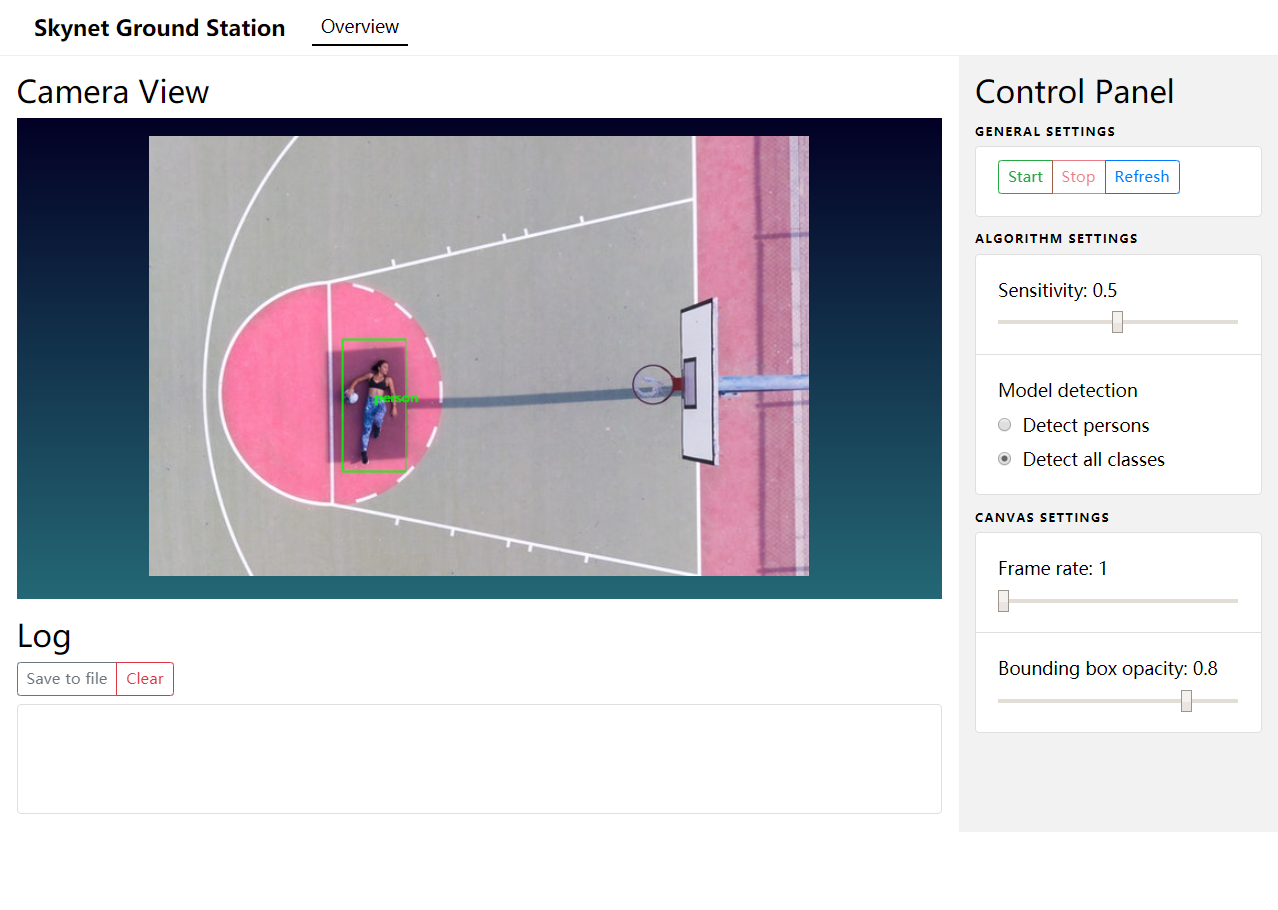
\includegraphics[width=15cm]{img/base_station.png}
\end{mdframed}
\caption{Screen Shot of the Web-app Running on the Base Station}
\label{basestationdiag}
\end{figure}

A web-application is used as the GUI for the base station. This allows for universal compatibility with all laptops, regardless of their operating system.

The base station hosts a Socket.IO server, and serves two clients: the PMB and the web-application. The server continuously queries the PMB for live video data and ML metadata results, and sends the data to the web-application for display.

The ML results are displayed as a bounding box around the detected object(s) in the frame (\textbf{F.BS.1}) and the type of the object detected is also displayed near the object (See Figure \ref{basestationdiag}). In particular, the ML results consist of three parts: the class of the detected object(s), the coordinates of the upper-left vertex of the bounding box(es), and the height/width of the bounding box(es).

The web application also displays real-time system status messages. These messages come from the PMB or the base station itself. The status updates include information on initiation or completion of processes, changes in PMB, PLB or base station settings, and system warnings/errors.

The base station continuously saves the received video and metadata locally for any analysis purposes (\textbf{F.BS.6}). All faults are also logged locally on the device to facilitate further debugging (\textbf{F.BS.5}).
%% maybe we just log all status messages, not limited to warnings/errors.

The user may use buttons and sliders on the web-application to adjust the visual properties of the web-application or change the settings on the PMB and PLB (\textbf{F.BS.2, F.BS.4}) such as the camera polling rate and ML sensitivity.

\subsubsection{Programming Libraries}

There are two JavaScript libraries used in both the client-side and server-side code of the base station.

The first library is \textit{socket.io}, which enables real-time, bidirectional and event-based communication between the browser and server. We use socket.io to establish a single communication protocol between the base station server and its clients. The client-side portion of the library is available in other languages such as C++ and Python with the same communication protocol, allowing for more versatility when programming the PMB to communicate with the base station. 

The second library is \textit{p5.js}, a client-side JavaScript framework that provides programmers with tools to create virtual canvases more easily. We use p5.js to draw live video feed and ML bounding box data; it allows for an elegant and high-level approach to programming this part of the web application.
